\begin{figure}[H]
 \centering 
 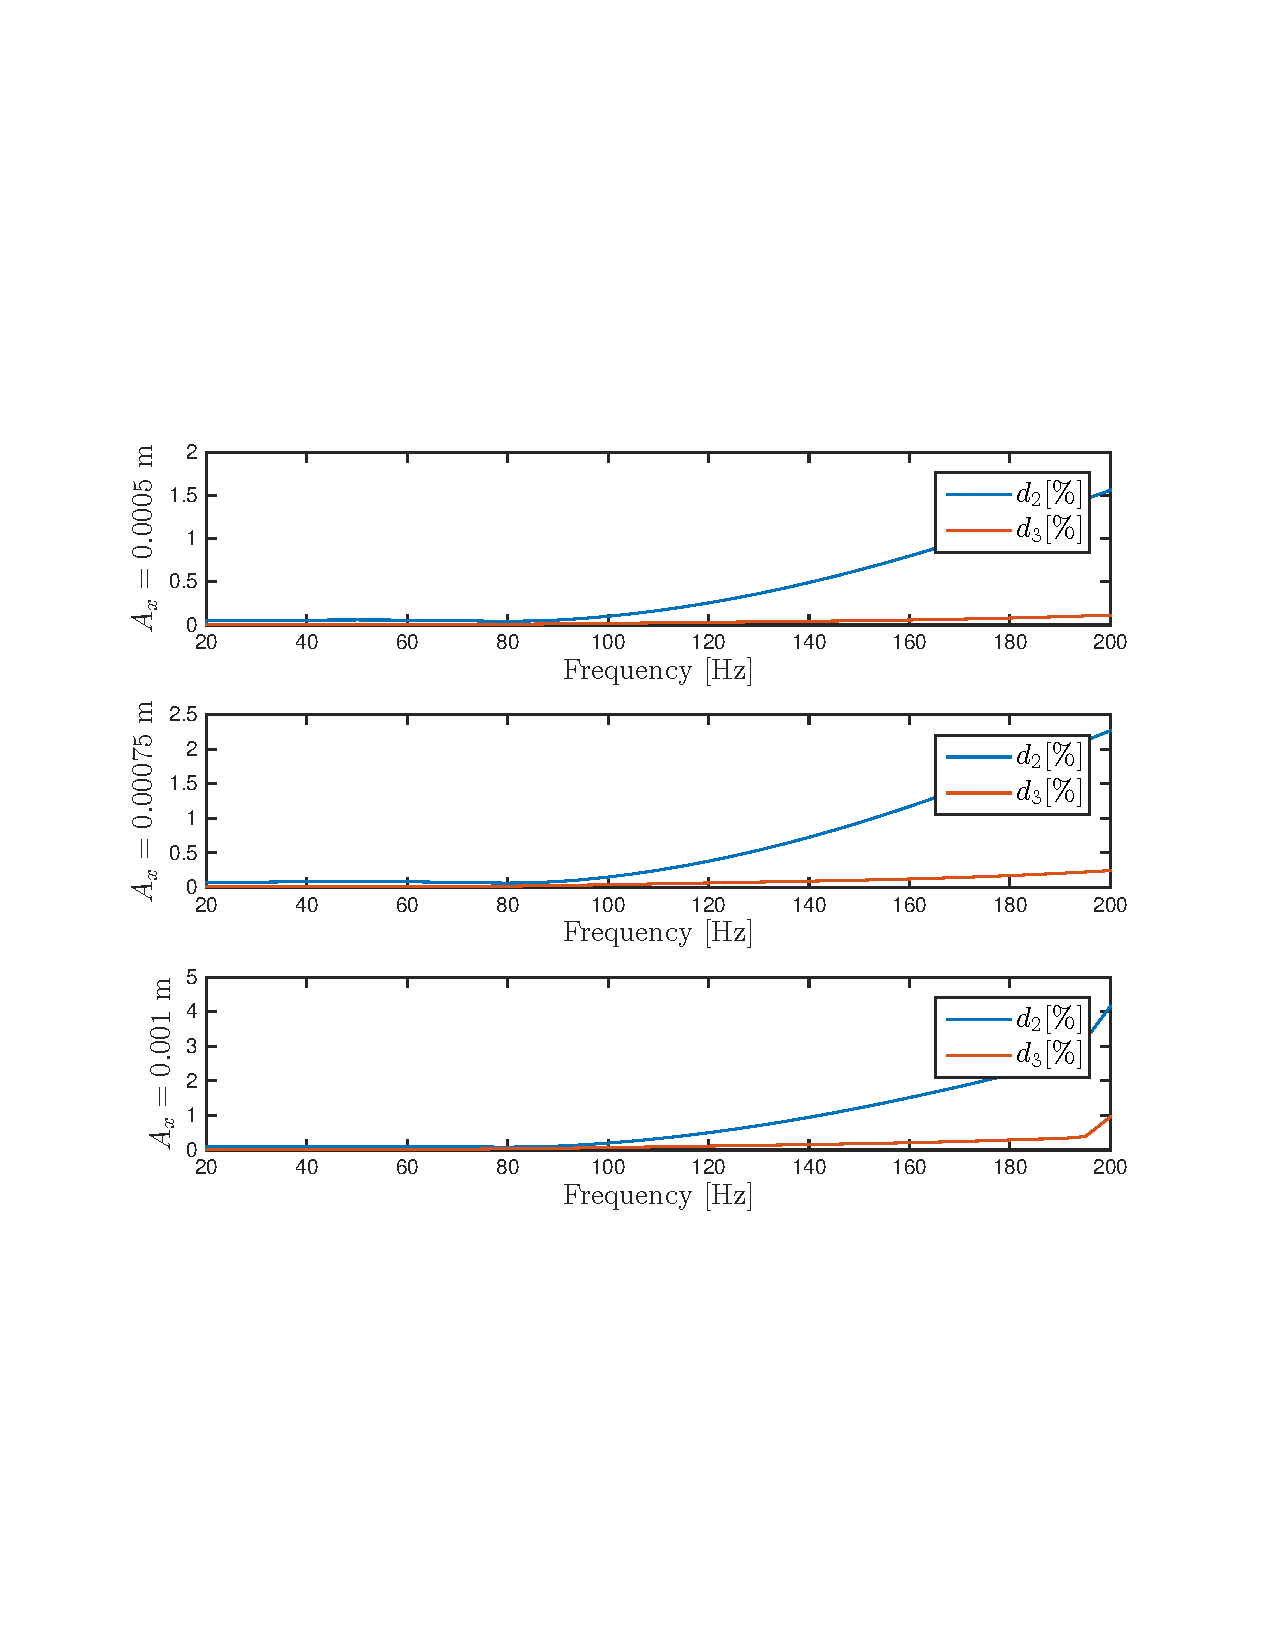
\includegraphics[trim=2cm 7cm 2cm 7cm, clip=true, totalheight=0.35\textheight, angle=0]{figures/P18d2d3.pdf}
 \caption{Effect of the variations of the frequency $f_c$ and the amplitude $A_x$ of the voice coil position $x_{ref}$ on the second and third order harmonic distortion}
 \label{fig:d2d3P18}
\end{figure}

In order to study the effect of the variations of the frequency $f_c$ and the amplitude $A_x$ of the voice coil position $x_{ref}$ on the second and third order harmonic distortions, we have computed $d_2$ and $d_3$ for a range of $A_x$ and $f_c$. The results can be seen on the figure \ref{fig:d2d3P18}. According to the graphic, the variations of the amplitude of the reference do not affect the shape of the distortion levels but their pourcentage, as it was the case in P5. On the other hand, in P5 the distortions levels were higher for 20 Hz than 200 Hz. It is the contrary in P18. That can be explained by the choice of the eigenvalues of the closed loop system. The controller is less effective around 200 Hz, that why the distortion levels are less attenuated. Finally we can notice that compared to P5, $d_2$ and $d_3$ have lower values and are close to 0\%, expecially $d_3$, which shows that the designed controller accomplishes its task, that is to say reducing the distortion effects.